\documentclass[dvipsnames,usenames,10pt]{beamer}

\usetheme{JuanLesPins}

\title{A Multi-Agent System for playing Briscola Chiamata} 

\author[B. Borja Fiz, F. De Santis, M. Gabarda]{Beltran Borja Fiz, Fabrizio De Santis, Marcos Gabarda}
\institute[Universitat Polit\`ecnica de Catalunya]{
			Multi-agent Systems Course\\
			Master in Artificial Intelligence\\
			Universitat Polit\`ecnica de Catalunya\\
			\texttt{\\ \{beltran.borja.fiz, fabrizio.de.santis, marcos.gabarda\}@est.fib.upc.edu}}
\date{\today}

\begin{document}

\frame{\titlepage}

\section*{Outline}

\frame{
	\frametitle{Outline}
  \begin{itemize}
   \item Problem Specification
   \vskip 2.0ex
   \item Analysis and Design Specification
   \begin{itemize}
    \item System Specification
    \item High level/Architectural Design
    \item Detailed Design
   \end{itemize}
   \vskip 2.0ex
   \item Implementation
   \begin{itemize}
      \item Prototype description
      \item Demo
   \end{itemize}
   \item Conclusions
  \end{itemize}
}

\part{Problem Specification}
\frame{\partpage}

\frame{
    \frametitle{Problem Specification}

  \begin{itemize}

   \item Chosen problem: the Briscola Chiamata card game
   \vskip 2.0ex
   \item Why the game is suitable for a multi-agents system?

%     \begin{itemize}  
%       \item Competitiveness and Cooperation.
%       \item Reactive and Proactive agents.
%       \item Could also have human players.
%     \end{itemize}

  \end{itemize}
}

\frame{
    \frametitle{A bit of terminology}
  
    \begin{itemize}
      \item Game: full play of the deck
      \vskip 2.0ex
      \item Round: subdivision of a game, each player play a card
      \vskip 2.0ex
      \item Trick: points collected in one round
      \vskip 2.0ex
      \item Suit: spades, hearts, diamonds, clubs
      \vskip 2.0ex
      \item Rank: 1-7, jack, queen, king
      \vskip 2.0ex
      \item Briscola (Brisca): a particular suit
    \end{itemize}
}

\frame{
    \frametitle{Briscola Chiamata}

    An italian card game of 5 players, 8 cards each (no cards undealt), 2 teams 

%Players look at cards and start bidding to be attempt to be the winner of the round. 
%Highest bidder then names a card (which he usually doesnt have) and the owner of that card becomes part of his team (only he knows... for now).
%So 2 teams. The person to reach a certain amount of points wins the game.

    \vskip 2.0ex

    Game in two-phases:
    \begin{itemize}  
      \item Bidding phase (amount of points to win the game)
      \item Playing phase
    \end{itemize}

    \vskip 2.0ex

    After the bidding phase, the briscola card is declared and the teams are formed.
}


\frame{
  \frametitle{Why is suitable for multi-agents system?}

  \begin{itemize}
    \item Uncertainity (nobody knows who are its team's partners)
    \item Sociality (needed in order to discover team settings)
    \begin{itemize}
      \item Cooperation (inside the team once partners are discovered)
      \item Competition (between opponent's teams)
      \item Trust/Reputation models needed 
    \end{itemize}
  \end{itemize}
	
  \vskip 2.0ex

  \begin{itemize}
    \item Main agent properties are satisfied
    \begin{itemize}
      \item Autonomy (players can be autonomous agents)
      \item Flexibility
      \begin{itemize}
	      \item Reactivity (players have to play when its their turn)
	      \item Proactivity (players can exchange information at any moment)
	      \item Social (players have to interact for discovering team settings)
      \end{itemize}
    \end{itemize}
  \end{itemize}
}

\part{System Specification}
\frame{\partpage}

\frame{
  \frametitle{System Specification}

  \begin{itemize}
    \item Analysis overview diagram: the interactions between the system and the environment
    \vskip 2.0ex
    \item Scenarios diagram: the dynamics of the game
    \vskip 2.0ex
    \item Goals overview diagram: how goals can be decomposed into subgoals
    \vskip 2.0ex
    \item System roles diagram: group different goals, percepts and actions under roles
  \end{itemize}
}

\frame[shrink,squeeze]{
  \frametitle{Analysis Overview Diagram}

  \begin{center}
    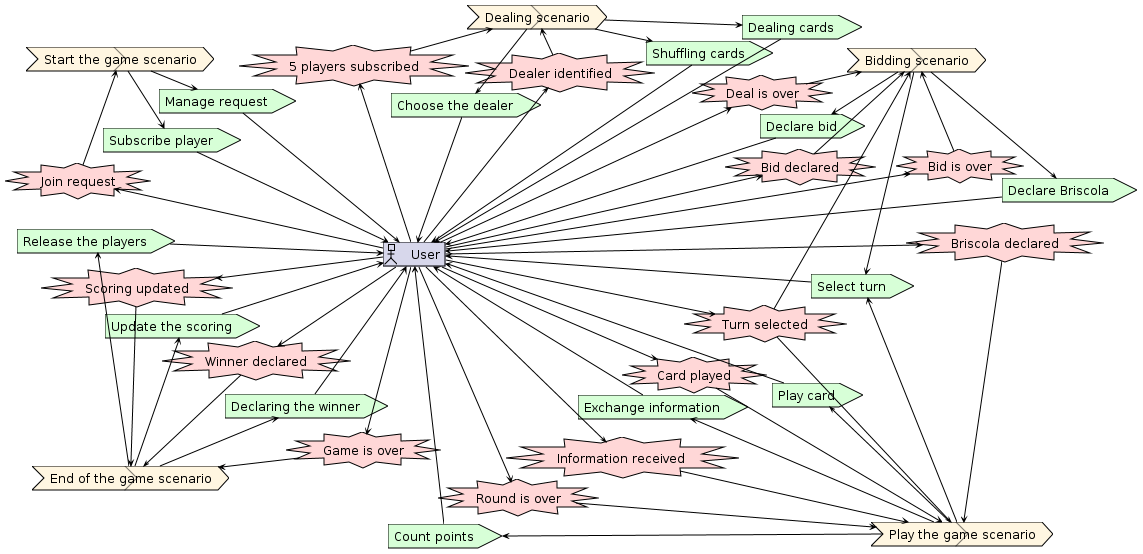
\includegraphics[keepaspectratio,scale=0.3]{pdt/images/system_specification/analysis_overview.png}
  \end{center}
}

\frame{
  \frametitle{Scenarios Diagram}

  \begin{center}
    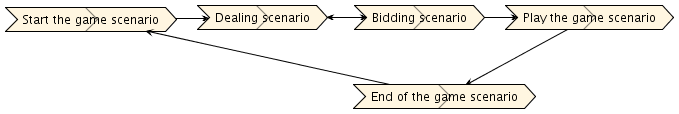
\includegraphics[keepaspectratio,scale=0.4]{pdt/images/system_specification/scenarios.png}
  \end{center}
}

\frame{
  \frametitle{Goals Overview Diagram}

  \begin{center}
    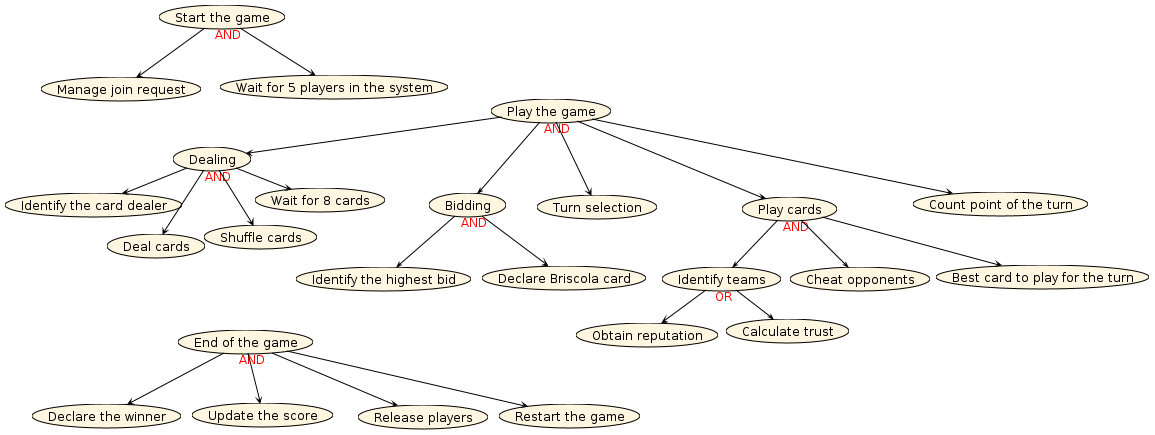
\includegraphics[keepaspectratio,scale=0.35]{pdt/images/system_specification/goal_overview.png}
  \end{center}
}

\frame[allowframebreaks]{
  \frametitle{System Roles Diagram}

  \begin{center}
    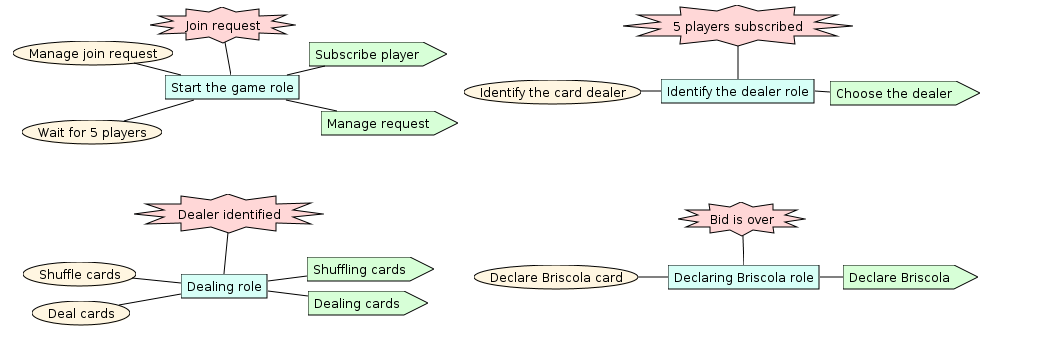
\includegraphics[keepaspectratio,scale=0.34]{fig/system_roles_1.png}
  \end{center}

  \break

  \begin{center}
    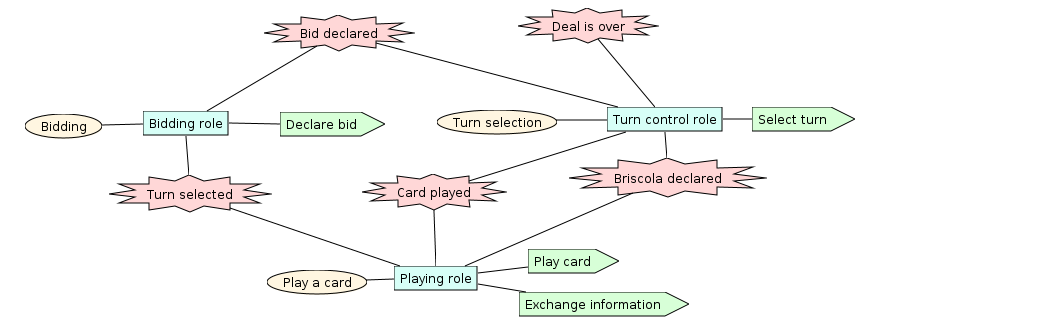
\includegraphics[keepaspectratio,scale=0.35]{fig/system_roles_2.png}
  \end{center}

  \break
  
  \begin{center}
    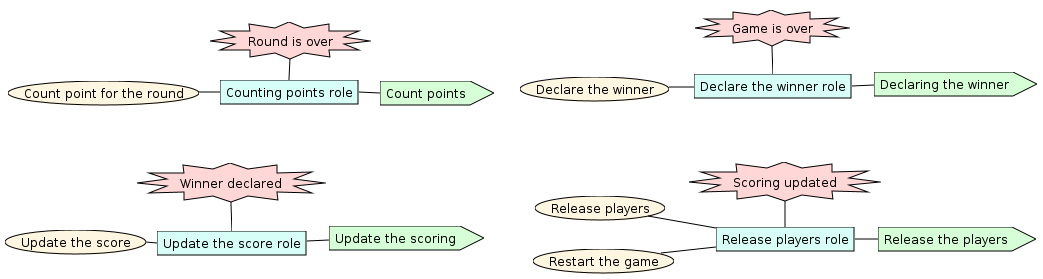
\includegraphics[keepaspectratio,scale=0.32]{fig/system_roles_3.png}
  \end{center}
}

\part{High-level/Architectural Design}
\frame{\partpage}

\frame{
  \frametitle{High-level/Architectural Specification}

  \begin{itemize}
    \item Data coupling diagram: links roles to data
    \vskip 2.0ex
    \item Agent-role grouping diagram: group the roles into agent types
    \vskip 2.0ex
    \item Agent acquaintance diagram: how agents interact with each's other
    \vskip 2.0ex
    \item System overview diagram: all agents in the system, along with their interface and interaction
  \end{itemize}
}

\frame{
  \frametitle{Data Coupling Diagram}

  \begin{center}
    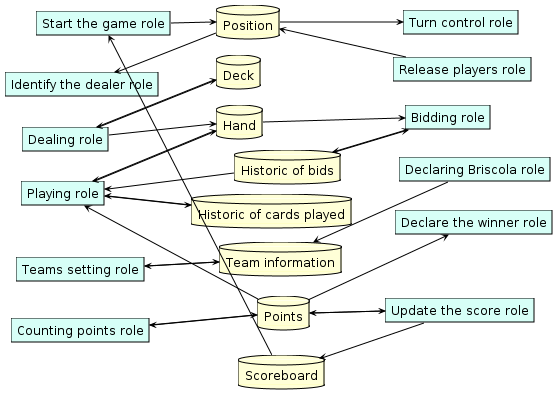
\includegraphics[keepaspectratio,scale=0.4]{pdt/images/architectural_design/data_coupling.png}
  \end{center}
}

\frame{
  \frametitle{Agent-Role Grouping Diagram}

  \begin{center}
    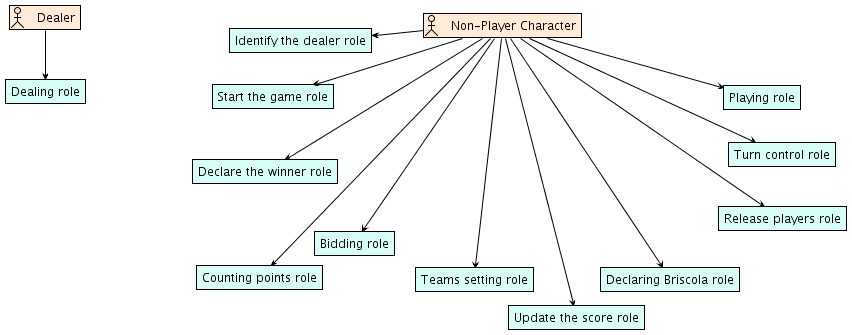
\includegraphics[keepaspectratio,scale=0.35]{pdt/images/architectural_design/aget-role_grouping.png}
  \end{center}
}

\frame{
  \frametitle{Agent Acquaintance Diagram}

  \begin{center}
    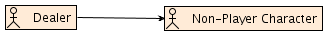
\includegraphics[keepaspectratio,scale=0.4]{pdt/images/architectural_design/agent_acquaintance.png}
  \end{center}
}

\frame{
  \frametitle{System Overview Diagram}

  \begin{center}
    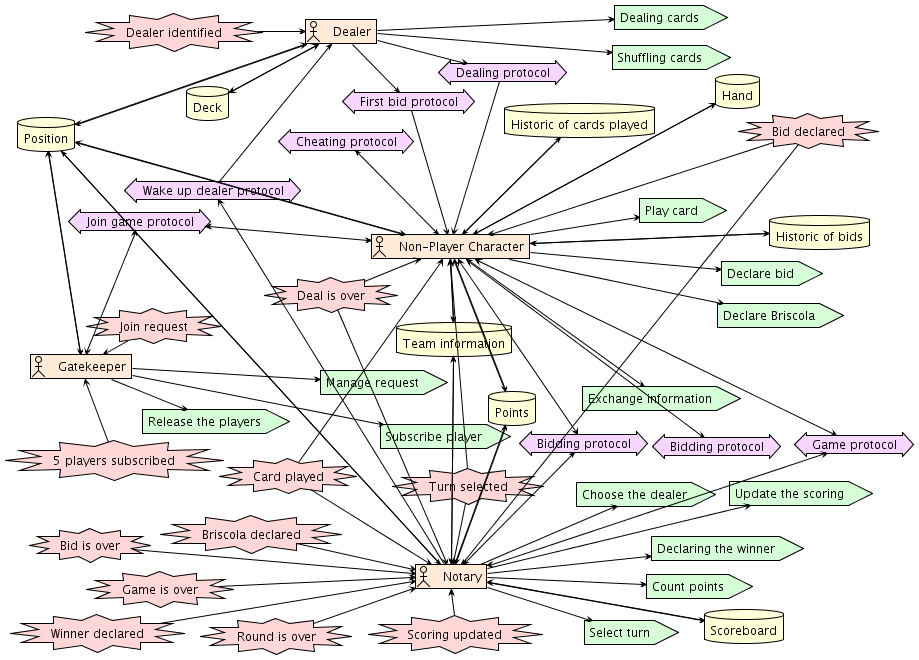
\includegraphics[keepaspectratio,scale=0.3]{pdt/images/architectural_design/system_overview.png}
  \end{center}
}

\frame[allowframebreaks]{
  \frametitle{Protocols}

  \begin{center}
  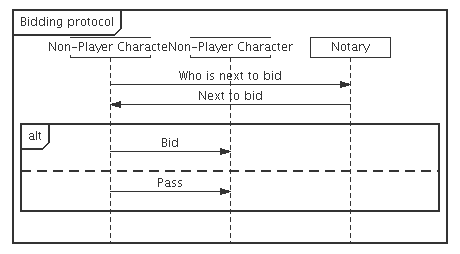
\includegraphics[keepaspectratio,scale=0.3]{pdt/images/protocols/Bidding_protocol.png}
  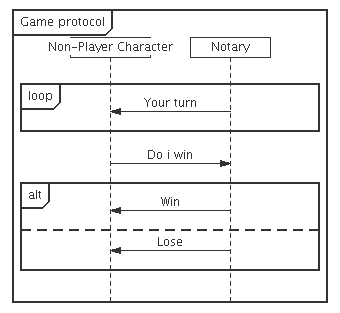
\includegraphics[keepaspectratio,scale=0.3]{pdt/images/protocols/Game_protocol.png}\\
  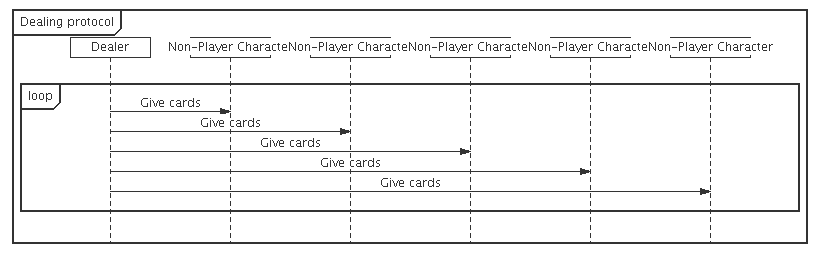
\includegraphics[keepaspectratio,scale=0.3]{pdt/images/protocols/Dealing_protocol.png}\\
  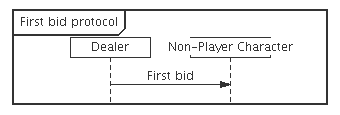
\includegraphics[keepaspectratio,scale=0.35]{pdt/images/protocols/First_bid_protocol.png}
  
\includegraphics[keepaspectratio,scale=0.35]{pdt/images/protocols/Wake_up_dealer_protocol.png}\\
  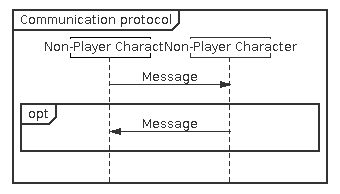
\includegraphics[keepaspectratio,scale=0.35]{pdt/images/protocols/Communication_protocol.png}
  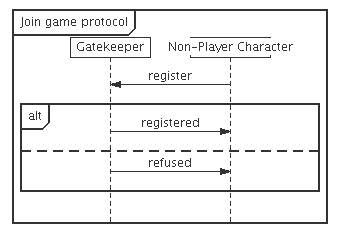
\includegraphics[keepaspectratio,scale=0.35]{pdt/images/protocols/Join_game_protocol.png}\\
  \end{center}

}

\part{Detailed Design}
\frame{\partpage}

\frame{
  \frametitle{Detailed Design}

  \begin{itemize}
    \item Agent overview diagrams: internals of agents
    \vskip 2.0ex
    \item Capability overview diagrams: internals of a capability in terms of plans or sub-capabilities and messages
  \end{itemize}
}

\frame{
  \frametitle{Agent Overview Diagram: gatekeeper agent}
  
  \begin{center}
    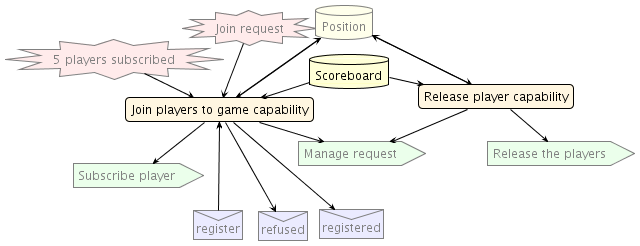
\includegraphics[keepaspectratio,scale=0.4]{pdt/images/detailed_design/gatekeeper_overview_diagram.png}
  \end{center}
}

\frame{
  \frametitle{Capability Overview Diagram: gatekeeper agent}
  \begin{center}
 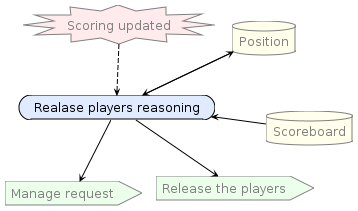
\includegraphics[keepaspectratio,scale=0.4]{pdt/images/detailed_design/release_player_capability_overview_diagram.png}
 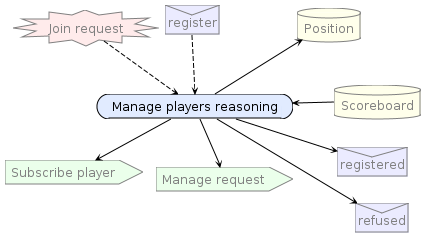
\includegraphics[keepaspectratio,scale=0.4]{pdt/images/detailed_design/join_players_capability_overview_diagram.png}
  \end{center}
}

\frame{
  \frametitle{Agent Overview Diagram: notary agent}
  
  \begin{center}
  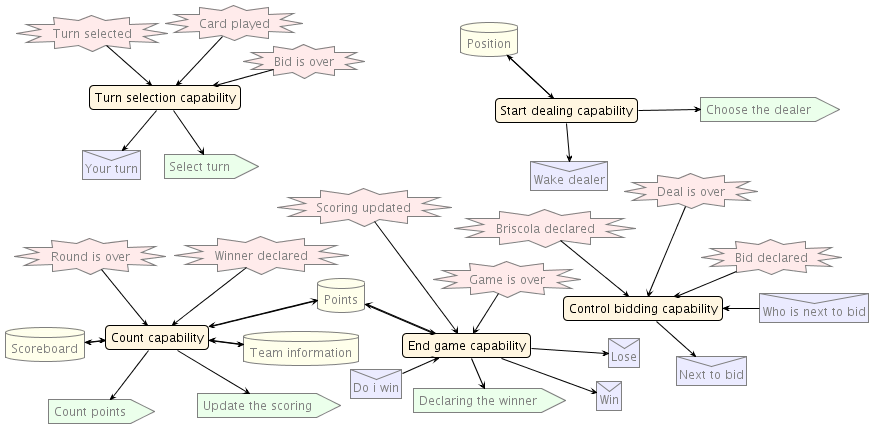
\includegraphics[keepaspectratio,scale=0.35]{pdt/images/detailed_design/notary_overview_diagram.png}
  \end{center}
}

\frame[allowframebreaks]{
  \frametitle{Capability Overview Diagram: notary agent}
  
  \begin{center}
  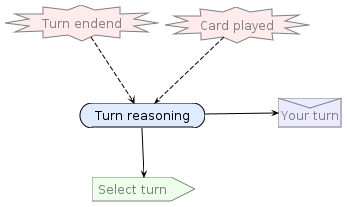
\includegraphics[keepaspectratio,scale=0.4]{pdt/images/detailed_design/turn_selection_capability_overview_diagram.png}
  
\includegraphics[keepaspectratio,scale=0.4]{pdt/images/detailed_design/end_the_game_capability_overview_diagram.png}\\
  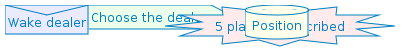
\includegraphics[keepaspectratio,scale=0.4]{pdt/images/detailed_design/start_dealing_capability_overview_diagram.png}
  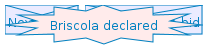
\includegraphics[keepaspectratio,scale=0.4]{pdt/images/detailed_design/control_bidding_capability_overview_diagram.png}\\
  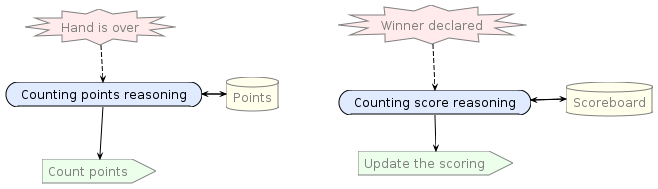
\includegraphics[keepaspectratio,scale=0.4]{pdt/images/detailed_design/count_points_capability_overview_diagram.png}
  \end{center}
}

\frame{
  \frametitle{Agent Overview Diagram: dealer agent}
  
  \begin{center}
  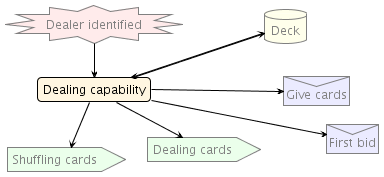
\includegraphics[keepaspectratio,scale=0.4]{pdt/images/detailed_design/dealer_overview_diagram.png}
  \end{center}
}

\frame{
  \frametitle{Capability Overview Diagram: dealer agent}
  
  \begin{center}
  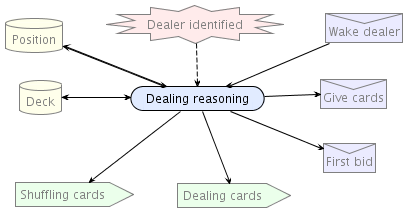
\includegraphics[keepaspectratio,scale=0.4]{pdt/images/detailed_design/dealing_capability_overview_diagram.png}
  \end{center}
}

\frame{
  \frametitle{Agent Overview Diagram: non-player-character agent}
  
  \begin{center}
  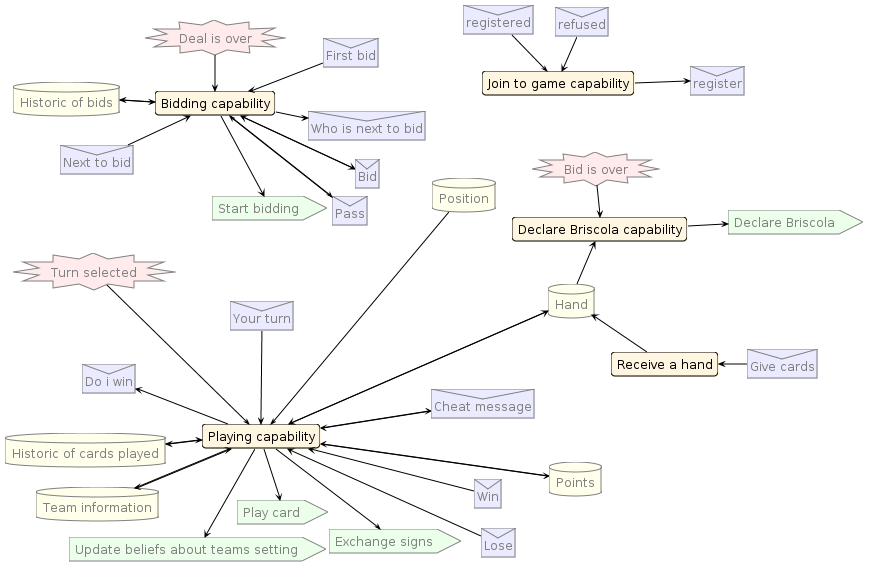
\includegraphics[keepaspectratio,scale=0.35]{pdt/images/detailed_design/non-player_character_overview_diagram.png}
  \end{center}
}

\frame[allowframebreaks]{
  \frametitle{Capability Overview Diagram: non-player-character agent}
  
  \begin{center}
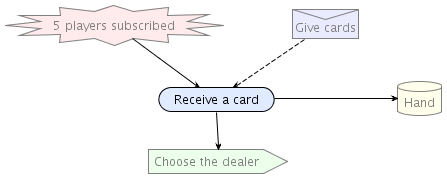
\includegraphics[keepaspectratio,scale=0.4]{pdt/images/detailed_design/receive_a_hand_capability_overview_diagram.png}
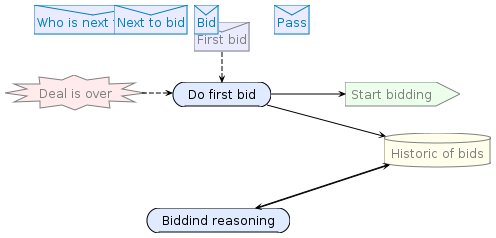
\includegraphics[keepaspectratio,scale=0.4]{pdt/images/detailed_design/bidding_capability_overview_diagram.png}\\
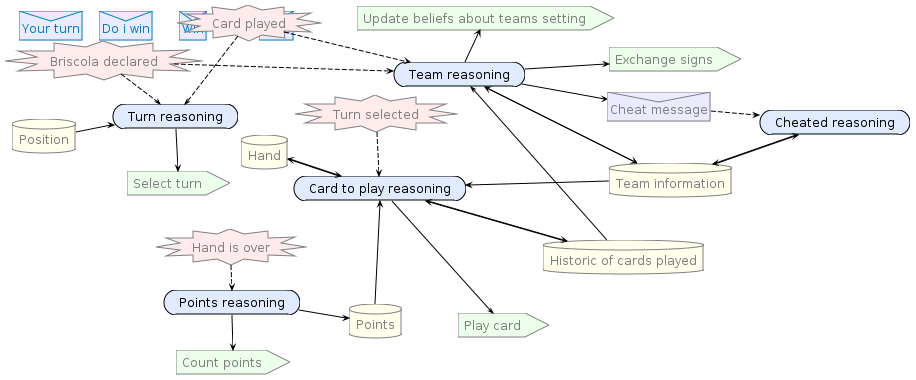
\includegraphics[keepaspectratio,scale=0.4]{pdt/images/detailed_design/playing_capability_overview_diagram.png}\\
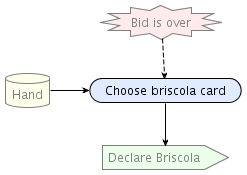
\includegraphics[keepaspectratio,scale=0.4]{pdt/images/detailed_design/declare_briscola_capability_overview_diagram.png}
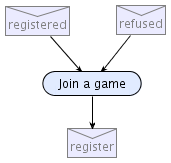
\includegraphics[keepaspectratio,scale=0.4]{pdt/images/detailed_design/join_to_game_capability_overview_diagram.png}
  \end{center}
}

\part{Implementation}
\frame{\partpage}

\frame{
  \frametitle{Prototype description}
  \begin{itemize}
    \item The prototype was built in two languages:
  \begin{itemize}
	\item Ennvironment was coded in Java (extension of a \texttt{apapl.Environment} class).
	\item Agents were coded in 2APL (founded in Prolog).
  \end{itemize}

	\item 2APL has little information on building environments so code inspection of an example was performed.
	\item The GUI was designed apart and then inserted into the environment.
  \end{itemize}
}


\frame{
  \frametitle{Prototype: concepts}
  \begin{itemize}
    \item The prototype is an approach of our Prometheus design of Briscola Chimiata applied to 2APL.
    \item We want ot test the develop of a real problem using 2APL platform.
    \item Cover all the scenarios, with the minimum functionalities.
    \item The GUI allows the designer of the agents to view how the agents play.
    %\item By showing the game steps at human eye sight speed, one could see the game in action instead of staring at a console.
    \item Fancy graphics were never intended, it is marely a visual aid, not an actual game to be played.
  \end{itemize}
}

\frame{
  \frametitle{Prototype : The future}
  \begin{itemize}
    \item Make agents more intelligent, adding learning algorithms or adding reputation models. 
    \item Personalize the strategies of each player, making competition.
    \item Allow human players to join, using and interface agent.
%%  Marcos: I comment this, because 2APL allows to use JADE, so other agents can be in other computers...
%   \item Or even more interesting, by adding the required libraries, one could potentially play on a server and have agents designed by different people play each other.
%   \item Due to lack of community this feature is unlikely to be added.
  \end{itemize}
}

\part{Demo}
\frame{\partpage}

\part{Conclusions}
\frame{\partpage}

\frame{
  \frametitle{Conclusions}

  \begin{columns}
    \begin{column}{0.5\textwidth}
      Good:
    \end{column}    
    \begin{column}{0.5\textwidth}
     Bad:
    \end{column}
  \end{columns}
  \begin{columns}
    \begin{column}{0.5\textwidth}
      \begin{itemize}
        \item Powerful mix of declarative (Prolog) and imperative programming style (Java)
        \item JADE platform compatibility.
        \item 2APL tools helpful during development.
      \end{itemize}
    \end{column}
    \begin{column}{0.5\textwidth}
     \begin{itemize}
      \item Lack of library to support agent side development
      \item Lack of a manual and examples
      \item Platform not at industry level 
     \end{itemize}
    \end{column}
  \end{columns}
}

\frame{
  \frametitle{EF($\Psi_1 \lor \Psi_2$)}

  \begin{itemize}
    \item $\Psi_1$: Finalize the prototype
    \vskip 2.0ex
    \item $\Psi_2$: Institute a contest
  \end{itemize}

  \vskip 4.0ex

  \begin{center}
  Join us at \url{http://2apl-upc-project.googlecode.com} !
  \end{center}
}


\begin{frame}{Bibliography}
\nocite{*}
\bibliographystyle{plain}
\bibliography{bc-pres}
\end{frame}

\end{document}
